
\begin{enumerate}
\item If you have a $9\myvolt$ voltage source, a blue LED, and a $500\myohm$ resistor all in series, how much current is running through the LED?
\item If you have a $3\myvolt$ voltage source and a red LED, what size resistor do you need to put in series with the LED to have it use $3\mymamp$ of current?
\item If you have a $10\myvolt$ voltage source, a blue LED, a red LED, and a $200\myohm$ resistor all in series, how much current is running through the LEDs?
\item If I have a $12\myvolt$ voltage source, a blue LED, and a red LED, and the LEDs have a maximum current of $30\mymamp$ before it breaks and a minimum current of $1\mymamp$ before it turns on, what range of resistors can I put in series with the LEDs to get them to light up without breaking?
\item In the circuit below, calculate the how much current flowing through each component and each component's voltage drop if R1 is $500\myohm$. \\ 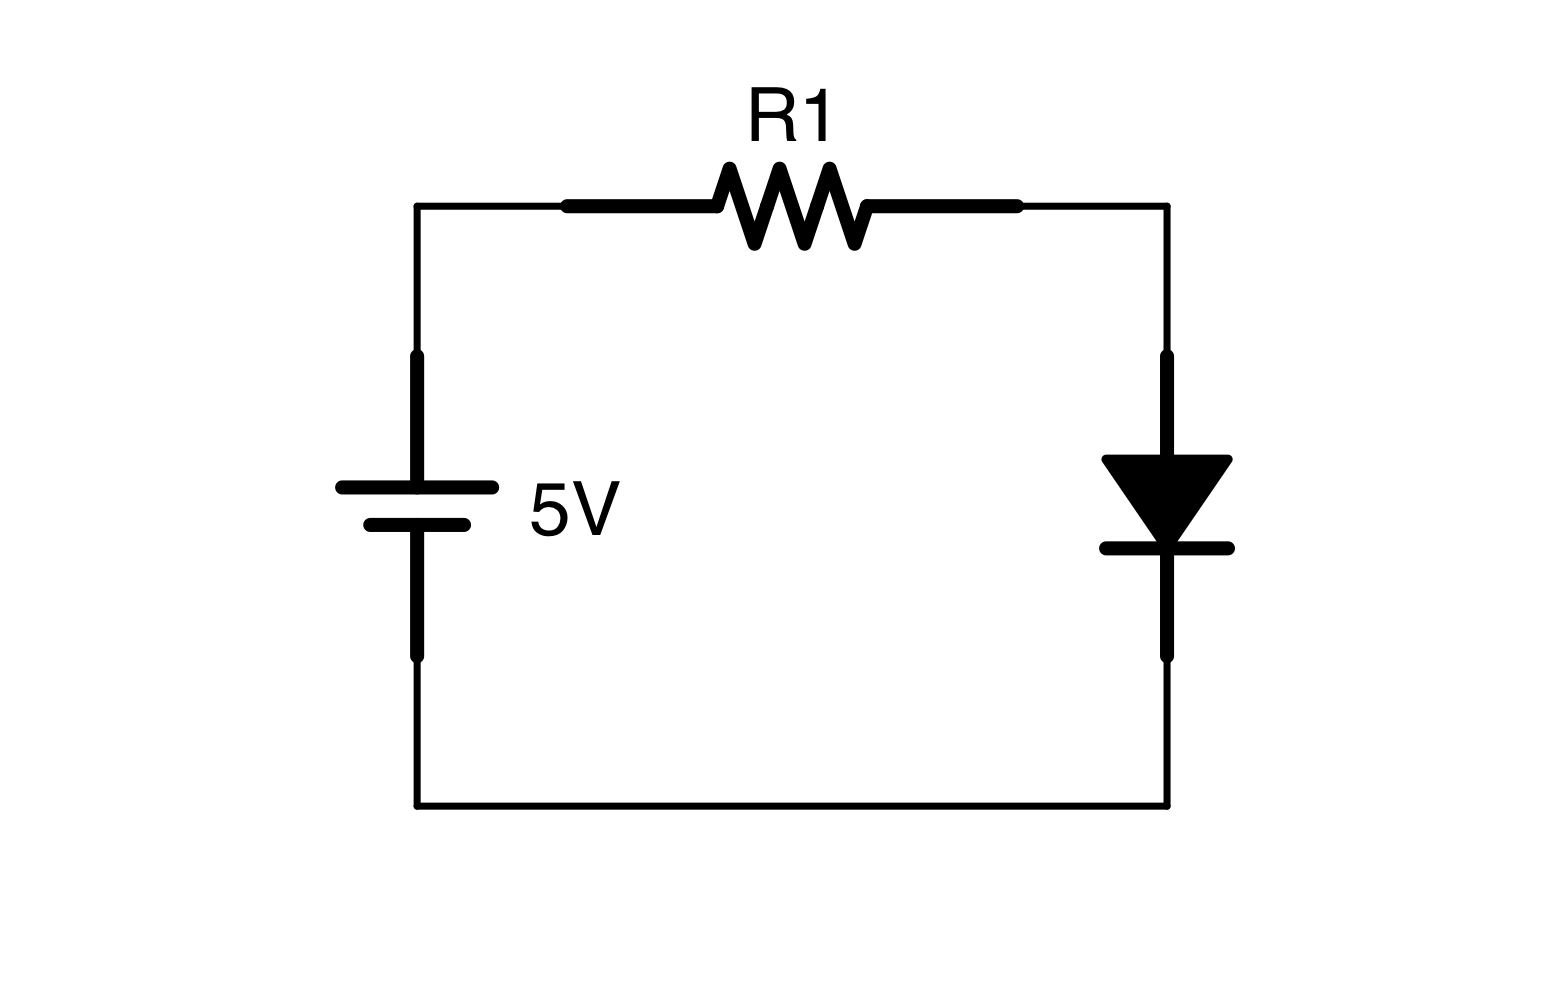
\includegraphics[scale=0.08]{DiodeApplyEx1.png}
\item Let's say instead of a standard diode, the diode is a blue LED.  Recalculate the current going through each component and the voltage drops for each component.
\item In the circuit below, calculate how much current is flowing through each component and each component's voltage drop if R1 is $300\myohm$, R2 is $400\myohm$, and R3 is $500\myohm$.  \\ 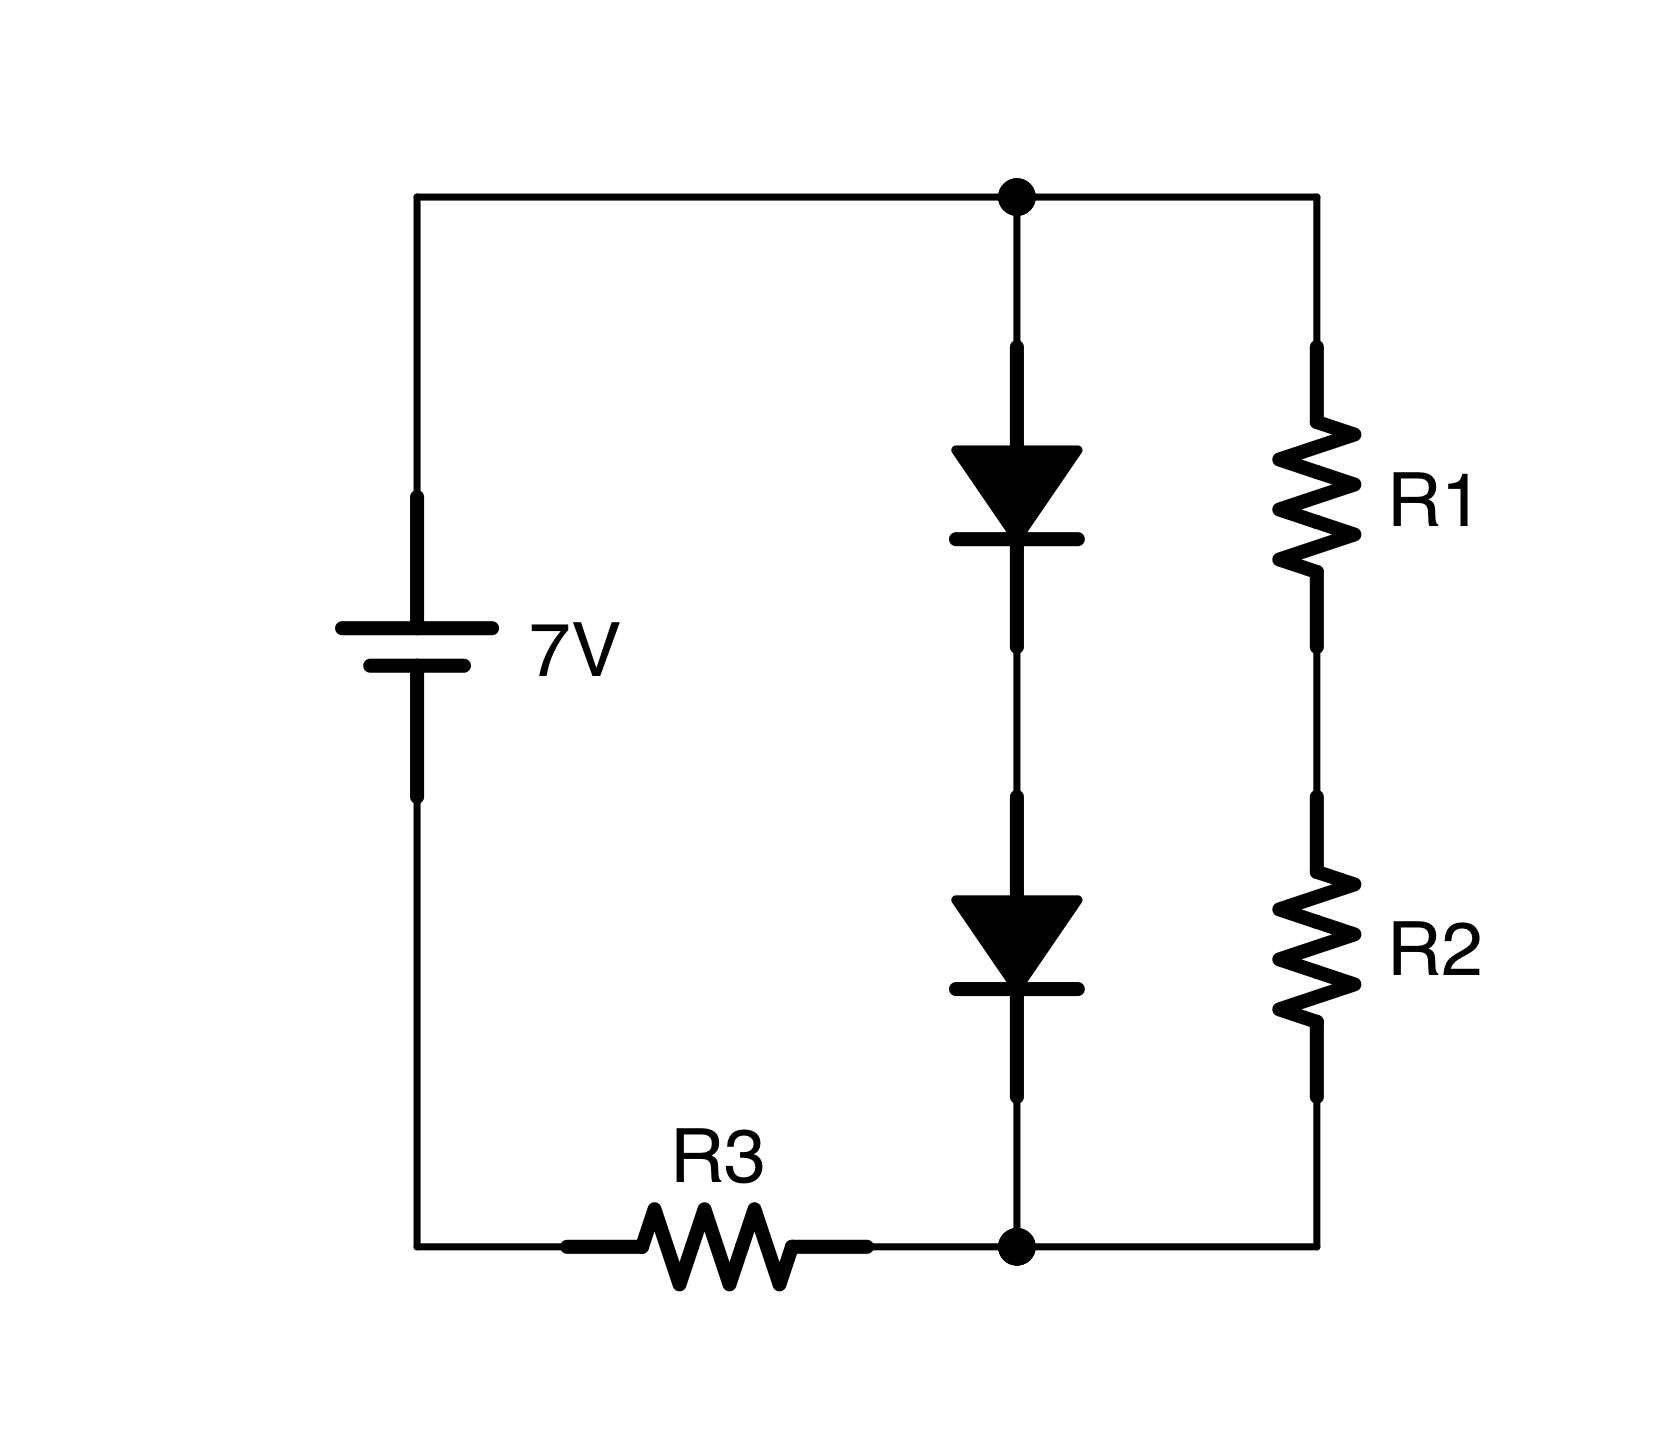
\includegraphics[scale=0.08]{DiodeApplyEx2.png}
\item Draw a circuit that provides a 6-volt regulated power supply to circuit load from a 9-volt battery using regular diodes.  Choose a resistor that works efficiently for a circuit load of $500\myohm$ and operates with a battery voltage from $7\myvolt$ to $9.6\myvolt$.  What is the current at the lowest and highest ranges of the battery?  How much is used by the circuit load and how much is wasted through the diodes in each configuration?
\item Draw an equivalent circuit to the previous question using a Zener diode instead of normal diodes.
\end{enumerate}
